\documentclass[aspectratio=169]{beamer} %[handout]
\mode<presentation>
\definecolor{links}{HTML}{0101DF}
\hypersetup{colorlinks,linkcolor=,urlcolor=links}
\setbeamercovered{transparent}
\usetheme[hideothersubsections]{Hannover}
\usecolortheme{fly}
\usenavigationsymbolstemplate{}
\usepackage{lmodern}
\renewcommand{\familydefault}{\sfdefault}

%%language
\usepackage[utf8]{inputenc}
\usepackage[T1]{fontenc}
\usepackage{ngerman}
\usepackage[ngerman,iso]{isodate}
%\usepackage{eurosym}
\hyphenation{}

\setbeamertemplate{section in toc}{\hspace*{1em}\inserttocsection}

\usepackage{graphicx}
\usepackage{multicol}

\definecolor{pm10}{HTML}{dcdcdc}
\definecolor{pm25}{HTML}{bcbcbc}
\definecolor{temp}{HTML}{B40404}
\definecolor{feuchte}{HTML}{0040FF}


\begin{document}
\title{Feinstaub in Lehrte}
\subtitle{Projektausschnitt von \href{http://www.luftdaten.info}{luftdaten.info}}
\author{Dr. H.-J. Dankert,\\S. Frenger}
\institute{luftdaten.info} 
\date{\today}

\frame{\titlepage} 

\begin{frame}{Inhalt}
  \begin{multicols}{2}
    \tableofcontents
  \end{multicols}
\end{frame}

\section{Feinstaub}

\subsection{Ursachen}
\begin{frame}{Ursachen}
  \begin{itemize}
  \item Verkehr
    \begin{itemize}
    \item Abgase
    \item Bremsen, auch von Zügen
    \item Stau, Umleitungsverkehr, Ferienverkehr
    \end{itemize}
  \item Heizung
  \item Pollen
  \item Feuer
  \item Nebel
  \item Ernte
  \item Baustelle
  \end{itemize}
\end{frame}

\subsection{Gesundheitsrisiken}
\begin{frame}{Gesundheitsrisiken}
  \begin{itemize}
  \item PM\textsubscript{10} kann in die Nasenhöhle
  \item PM\textsubscript{2,5} kann in Bronchien und Lungenbläschen
  \item noch kleinere in Lungengewebe und Blutkreislauf
  \item Herz-Kreislauf-Erkrankungen
  \item Asthma, Atemnot, Atemwegserkrankungen
  \item Bluthochdruck, Herzinfarkt, Herzrhythmusstörung
  \end{itemize}
\end{frame}

\subsection{Gesetz}
\begin{frame}{Gesetz}
  \begin{itemize}
  \item \href{https://www.umweltbundesamt.de/daten/luft/feinstaub-belastung}{umweltbundesamt.de}
  \item PM\textsubscript{10} von 50 $\mu$g/m\textsuperscript{3} im Tagesmittel 35x im Jahr überschritten werden.
  \item EU-Grenzwert 40 $\mu$g/m\textsuperscript{3} ist Jahresmittel
  \item WHO-Grenzwert 20 $\mu$/gm\textsuperscript{3} ist Jahresmittel
  \end{itemize}
\end{frame}

\subsection*{Medien}
\begin{frame}{Aktuelle Nachrichten}
  \begin{itemize}
  \item 17-07-27 Augsburger \href{http://www.augsburger-allgemeine.de/panorama/In-Stuttgart-droht-jetzt-ein-Diesel-Fahrverbot-id42204121.html}{Stuttgart droht Diesel-Fahrverbot}
  \item 17-09-16 Wirtschaftsnachrichten \href{https://deutsche-wirtschafts-nachrichten.de/2017/09/16/feinstaub-belastung-vielen-staedten-drohen-fahrverbote/}{Vielen Städten droht Fahrverbot}
  \item 17-09-19 Euronews \href{http://de.euronews.com/2017/09/19/der-deutsche-autowahlkampf}{Deutscher Autowahlkampf}
  \item 17-11-06 Stadt Lehrte referenziert \href{http://piratenpartei-lehrte.de/2017/09/11/feinstaub-in-lehrte/}{Projekt} im Umweltbericht
  \item 18-01-04 Silvester \href{https://sbamueller.wordpress.com/2018/01/01/silvester-und-feinstaub/}{Animation}
  \item 18-01-18 Welt \href{https://www.welt.de/wirtschaft/article172580444/Fahrverbote-kann-Deutschland-kaum-noch-verhindern.html}{Fahrverbote in Deutschland kaum zu verhindern}
  \end{itemize}
\end{frame}

\section{Lehrte}
\subsection*{Lehrte}
\begin{frame}{Interessant für Lehrte?}
  \begin{itemize}
  \item Interpolation Messstellen Hannover und Braunschweig fragwürdig:
  \item Nähe zu Bundesautobahn
  \item Nähe zu Autobahnkreuz
  \item Nähe zu Bahngleisen
  \item Kleingärten im Stadtkern ``überbauen''?
  \item Bewusstsein um Feinstaub wächst
  \item ISEK: Innen- vor Außenbebauung hinterfragen?
  \end{itemize}
\end{frame}

\subsection{Quellen}
\begin{frame}{Quellen}
  \begin{itemize}
  \item \href{http://luftdaten.info/}{luftdaten.info}, \href{https://archive.luftdaten.info/}{archiv}
  \item \href{https://www.umwelt.niedersachsen.de/themen/luft/luen/aktuelle_messwerte/archiv/download/}{umwelt.niedersachsen.de Luft Download Archiv}
  \item \href{www.bund-neckar-alb.de/fileadmin/rv_neckar-alb/MasterarbeitBlonFeinstaubmessungimVergleich2017.pdf}{Messprinzip Masterarbeit}
  \item \href{www.analyticjournal.de/fachreports/grimm_nano_tubln_07_09/grimm_nano_pesch.pdf}{analyticjornal.de}
  \item \href{https://www.lanuv.nrw.de/fileadmin/lanuv/gesundheit/schadstoffe/gesundheitliche_wirkungen.pdf}{lanuv.nrw.de}
  \end{itemize}
\end{frame}

\section{luftdaten.info}
\subsection{Stuttgart}
\begin{frame}{Stuttgart}
  \begin{itemize}
  \item Projekt luftdaten.info
  \item Feinstaub selber messen
  \item offizielles Messen ist teuer, also messen wir selbst:
  \item Stuttgart im Tal
  \item \href{https://de.wikipedia.org/wiki/Open_Data}{Open Data}
  \item Projektstart 2015
  \end{itemize}
\end{frame}

\subsection{Bausatz}
\begin{frame}{\href{http://luftdaten.info/feinstaubsensor-bauen/}{Einsteiger-Bausatz}}
  \begin{itemize}
  \item MiniPC mit WLAN: NodeMCU ESP8266
  \item Feinstaubsensor: SDS011
  \item Temperatur \& Luftfeuchte: DHT22
  \item Wetterschutz: HT Bogen
  \item Verbindung: USB-Ladekabel, WLAN
  \end{itemize}
  \begin{center}
    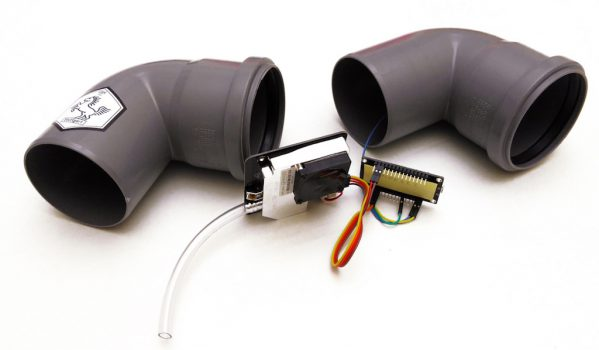
\includegraphics[width=6cm]{../screenshots/Feinstaub-Sensor-Bausatz-e1479558693357.jpg}
  \end{center}
\end{frame}

\subsection{Teilnehmer}
\begin{frame}{Teilnehmer}
heute etwa 15 Sensoren in Lehrte, > 40 mit Hannover und Braunschweig
  \begin{itemize}
  \item Aktionsbündnis Lehrter Laubenpieper
  \item DIE LINKE. Lehrte/Sehnde
  \item Piratenpartei Lehrte
  \item Siedlergemeinschaft Hohnhorst Lehrte e.V.
  \item weitere Anlieger
  \end{itemize}
  \begin{center}
    \includegraphics[width=6cm]{../screenshots/IMG_20170902_164405.jpg}
  \end{center}
\end{frame}

\section{Schnappschuss}
\subsection{Europa}
\begin{frame}{Europa \href{http://hannover.maps.luftdaten.info/\#5/52.373/10.005}{luftdaten.info} 2018-01-20 09:00}
  \begin{center}
    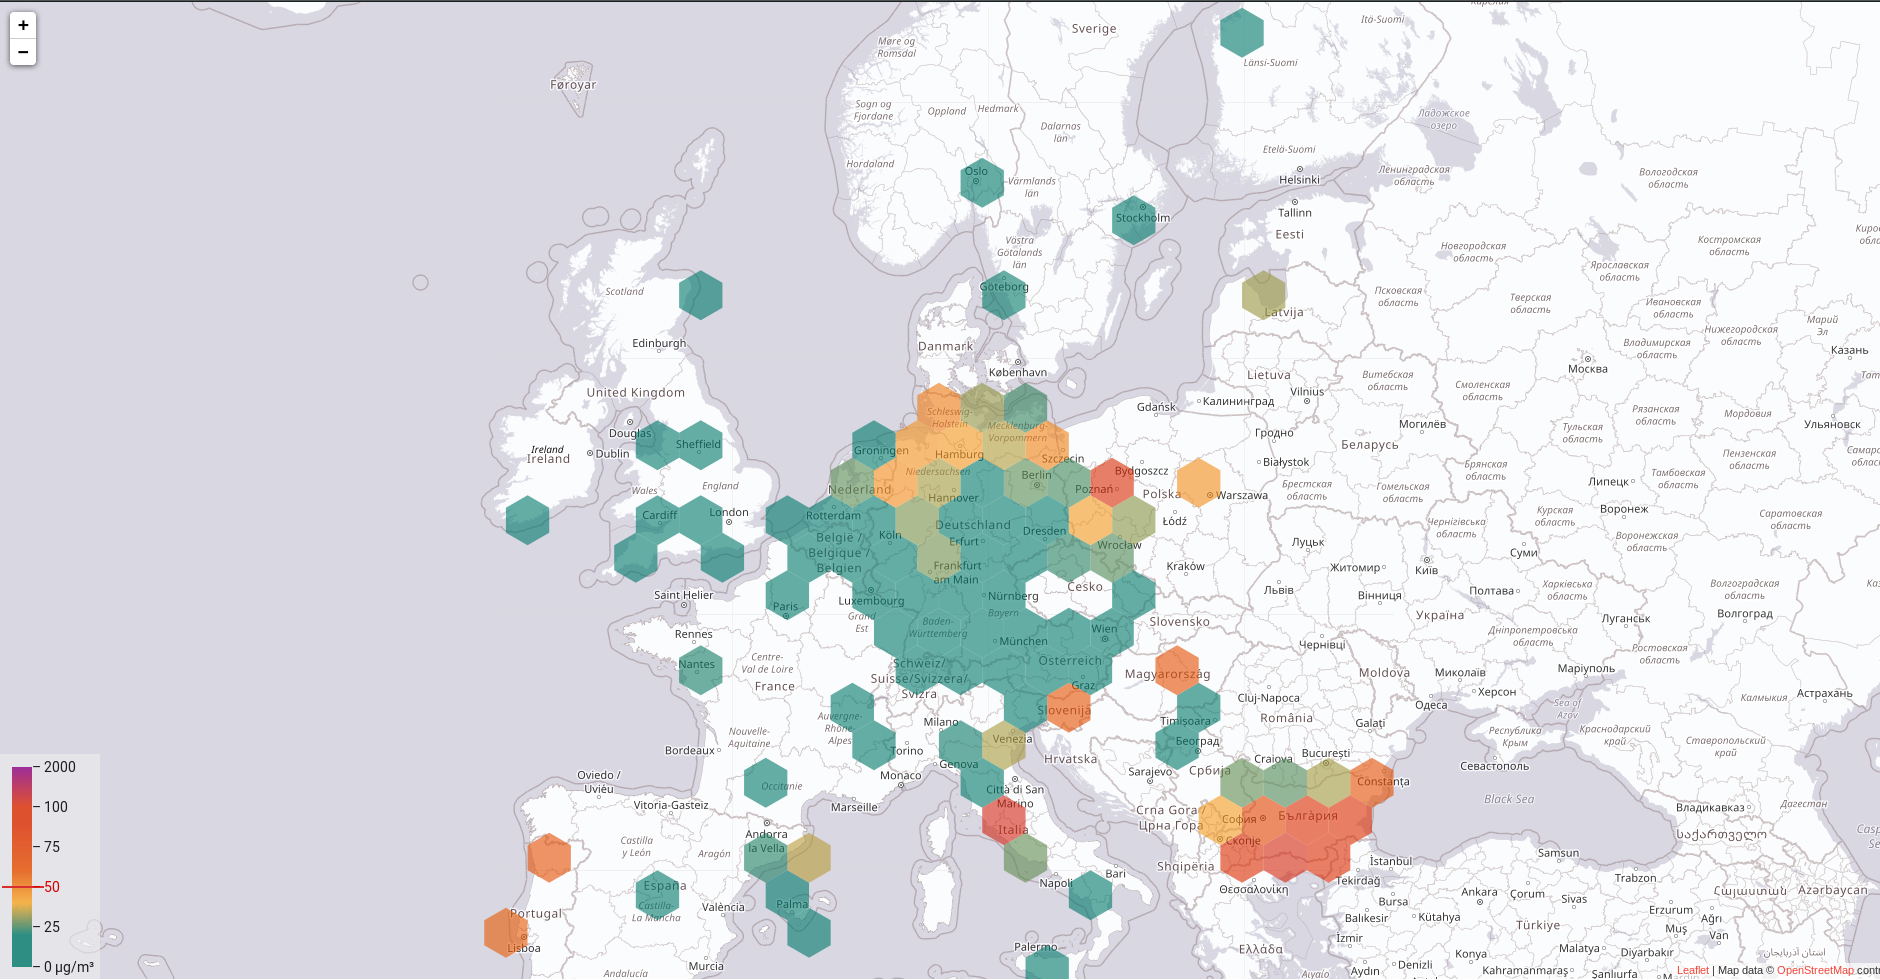
\includegraphics[width=\textwidth]{../screenshots/luftdaten-zoom-e.png}
  \end{center}
\end{frame}
\subsection{Deutschland}
\begin{frame}{Deutschland \href{http://hannover.maps.luftdaten.info/\#6/52.373/10.005}{luftdaten.info} 2018-01-20 09:00}
  \begin{center}
    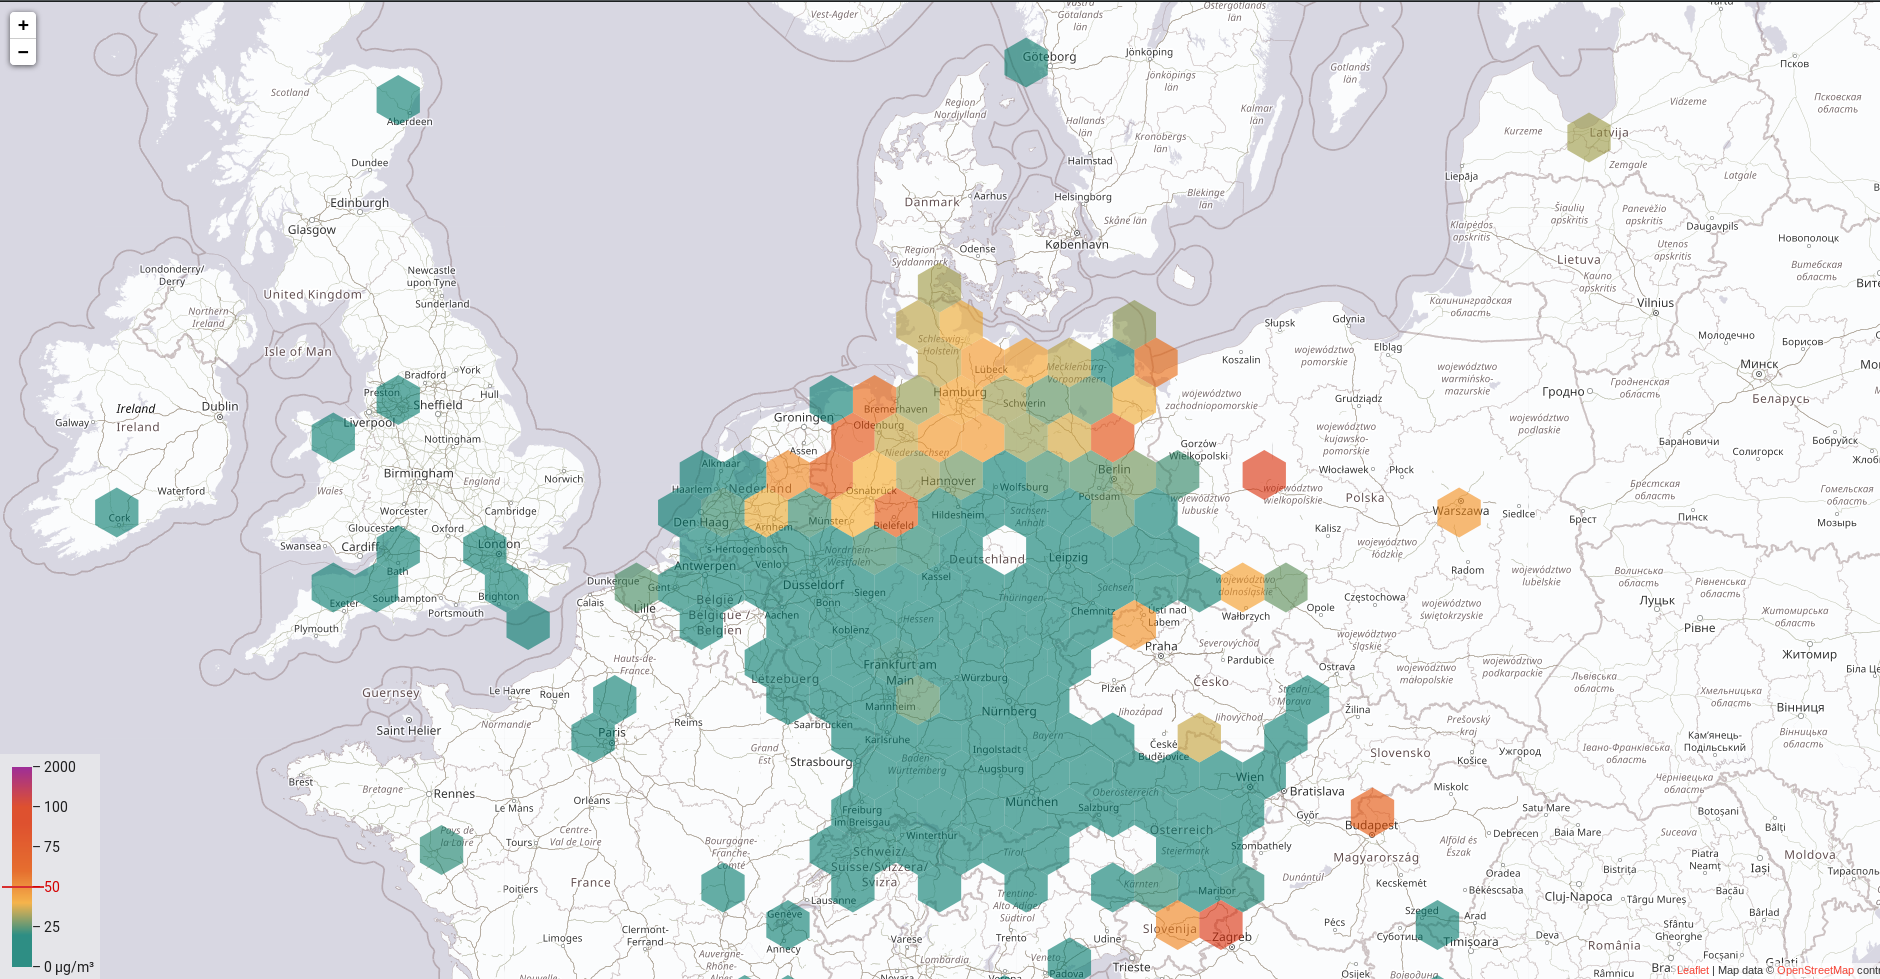
\includegraphics[width=\textwidth]{../screenshots/luftdaten-zoom-f.png}
  \end{center}
\end{frame}
\subsection*{der Norden}
\begin{frame}{der Norden \href{http://hannover.maps.luftdaten.info/\#8/52.373/10.005}{luftdaten.info} 2018-01-20 09:00}
  \begin{center}
    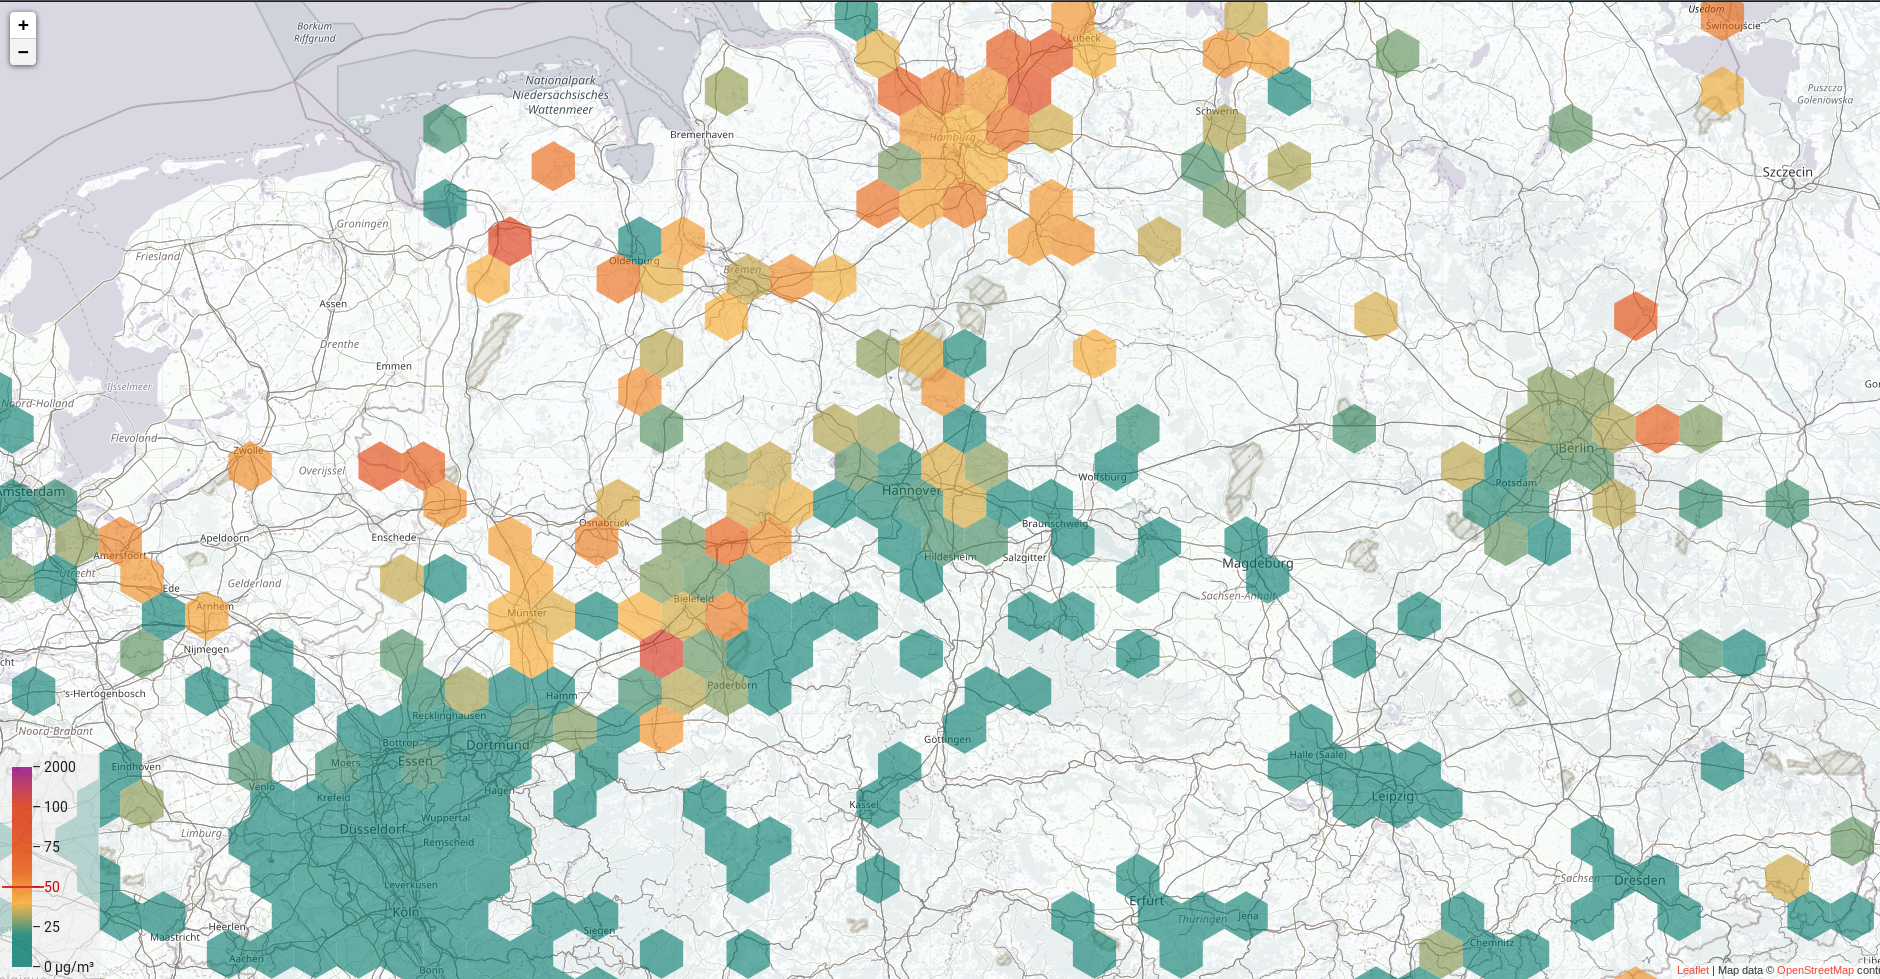
\includegraphics[width=\textwidth]{../screenshots/luftdaten-zoom-d.png}
  \end{center}
\end{frame}
\subsection{Hannover}
\begin{frame}{Hannover \href{http://hannover.maps.luftdaten.info/\#10/52.373/10.005}{luftdaten.info} 2018-01-20 09:00}
  \begin{center}
    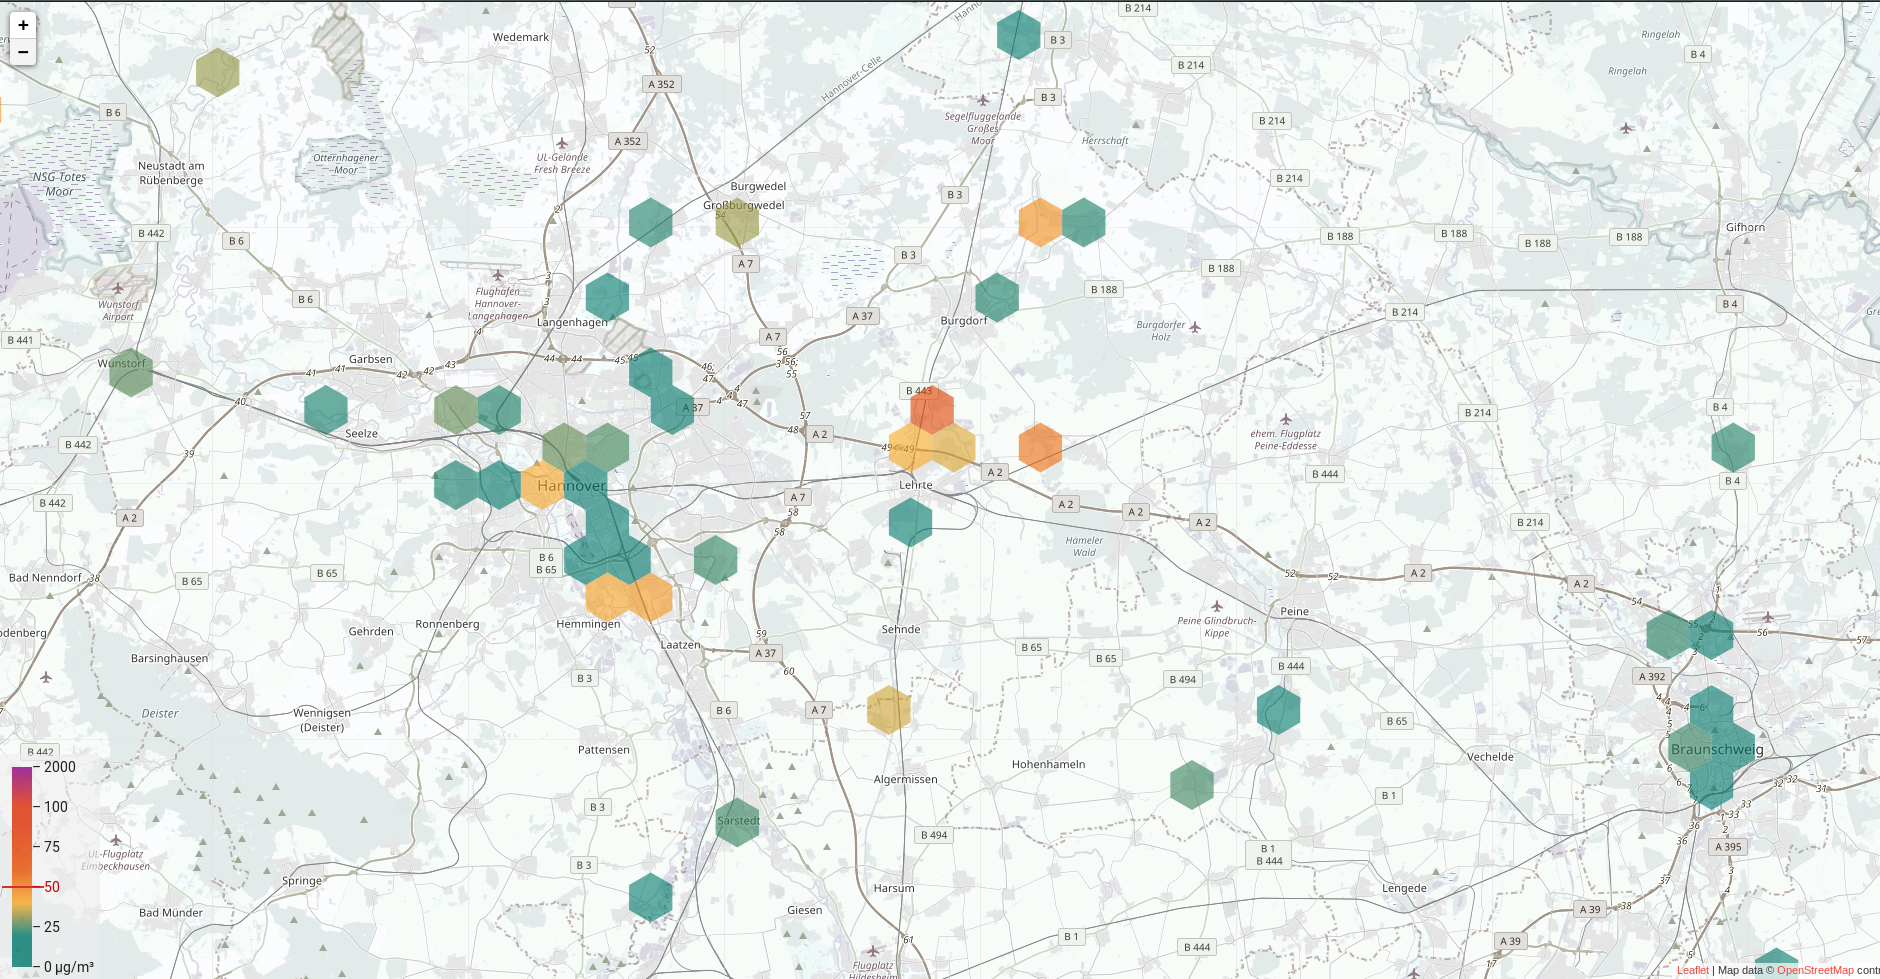
\includegraphics[width=\textwidth]{../screenshots/luftdaten-zoom-b.png}
  \end{center}
\end{frame}
\subsection{Lehrte}
\begin{frame}{Lehrte \href{http://hannover.maps.luftdaten.info/\#12/52.373/10.005}{luftdaten.info} 2018-01-20 09:00}
  \begin{center}
    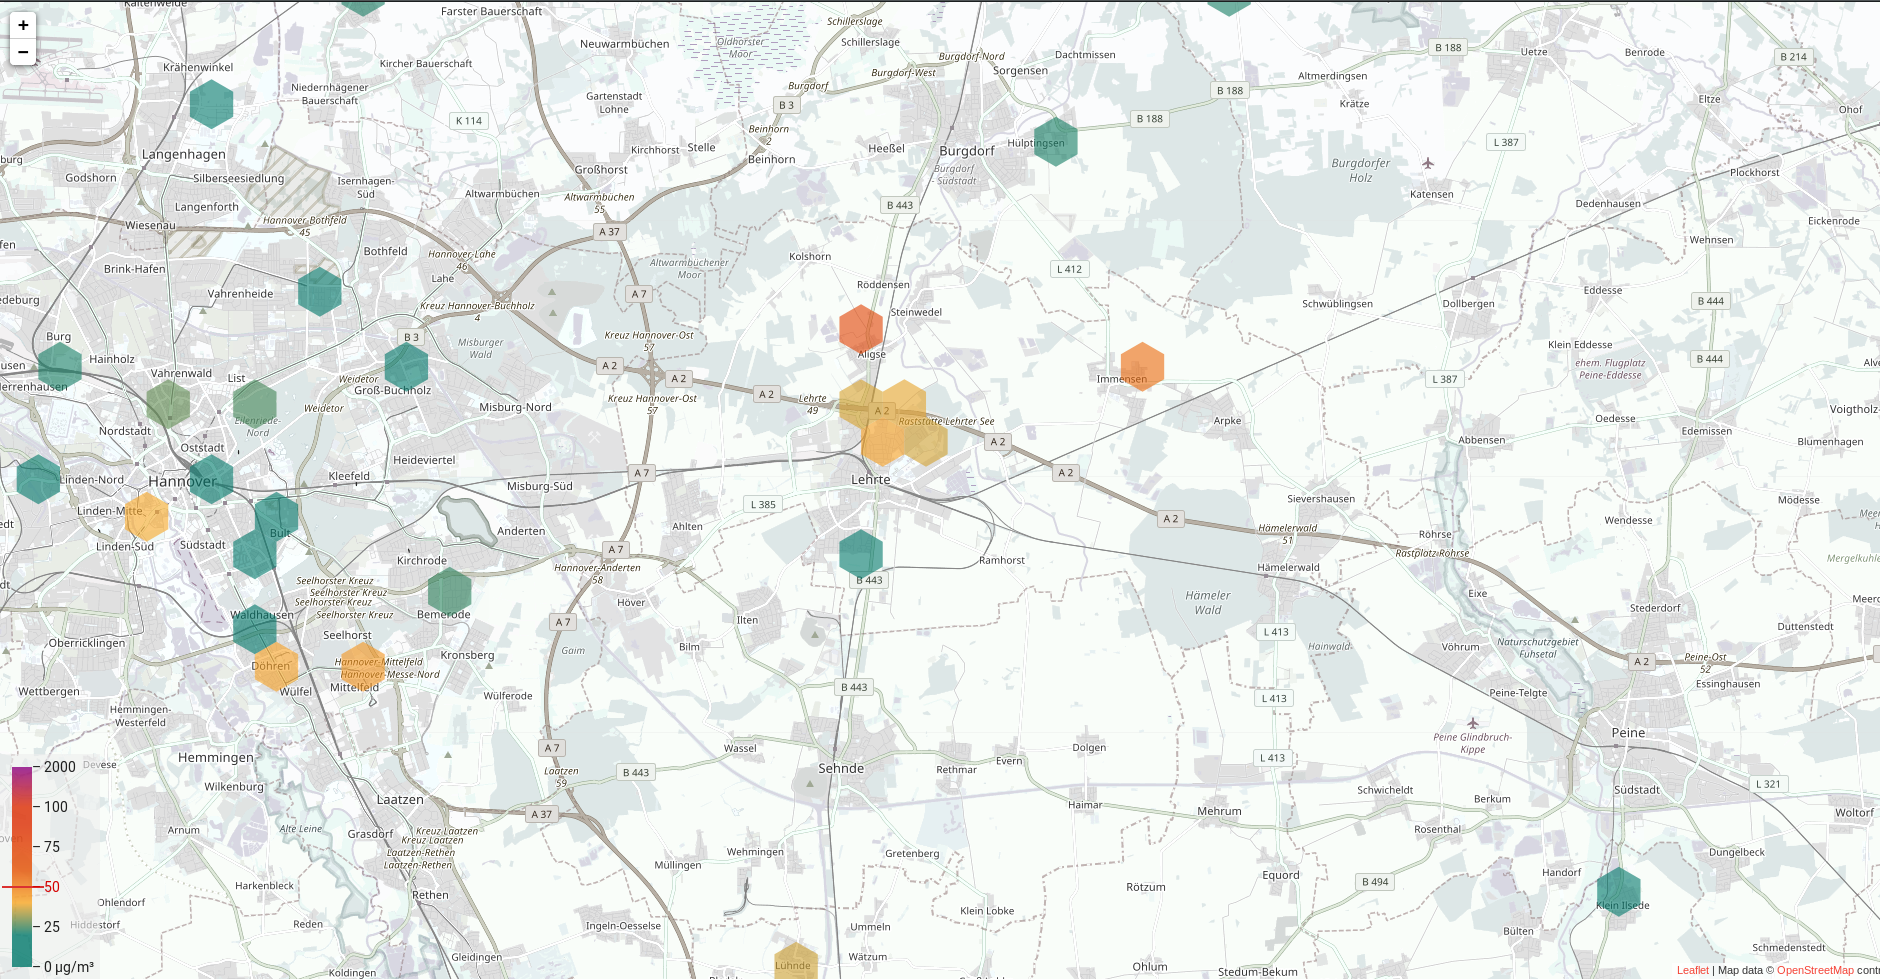
\includegraphics[width=\textwidth]{../screenshots/luftdaten-zoom-a.png}
  \end{center}
\end{frame}

\section{Historie}
\subsection*{Historie}
\begin{frame}{Gruppierung}
  \begin{itemize}
  \item Gruppierung der Sensoren
    \begin{itemize}
    \item Braunschweig
    \item Hannover
    \item Lehrte
    \end{itemize}
  \item Zeitachse in Monaten
    \begin{itemize}
    \item September
    \item ...
    \item Januar
    \end{itemize}
  \item Werte
    \begin{itemize}
    \item \textcolor{pm10}{PM\textsubscript{10} (luftdaten.info + GAA)}
    \item \textcolor{pm25}{PM\textsubscript{2,5}}
    \item \textcolor{temp}{Temperatur}
    \item \textcolor{feuchte}{Luftfeuchtigkeit (luftdaten.info + GAA)}
    \end{itemize}
  \end{itemize}
\end{frame}

\subsection{September}
\begin{frame}{Braunschweig September 2017}
  \begin{center}
    \includegraphics[width=\textwidth]{../png/2017-09-bs.png}
  \end{center}
\end{frame}
\begin{frame}{Hannover \hspace{4cm} September 2017}
  \begin{center}
    \includegraphics[width=\textwidth]{../png/2017-09-h.png}
  \end{center}
\end{frame}
\begin{frame}{Lehrte \hspace{2cm} September 2017}
  \begin{center}
    \includegraphics[width=\textwidth]{../png/2017-09-l.png}
  \end{center}
\end{frame}

\subsection{Oktober}
\begin{frame}{Braunschweig Oktober 2017}
  \begin{center}
    \includegraphics[width=\textwidth]{../png/2017-10-bs.png}
  \end{center}
\end{frame}
\begin{frame}{Hannover \hspace{4cm} Oktober 2017}
  \begin{center}
    \includegraphics[width=\textwidth]{../png/2017-10-h.png}
  \end{center}
\end{frame}
\begin{frame}{Lehrte \hspace{2cm} Oktober 2017}
  \begin{center}
    \includegraphics[width=\textwidth]{../png/2017-10-l.png}
  \end{center}
\end{frame}

\subsection{November}
\begin{frame}{Baunschweig November 2017}
  \begin{center}
    \includegraphics[width=\textwidth]{../png/2017-11-bs.png}
  \end{center}
\end{frame}
\begin{frame}{Hannover \hspace{4cm} November 2017}
  \begin{center}
    \includegraphics[width=\textwidth]{../png/2017-11-h.png}
  \end{center}
\end{frame}
\begin{frame}{Lehrte \hspace{2cm} November 2017}
  \begin{center}
    \includegraphics[width=\textwidth]{../png/2017-11-l.png}
  \end{center}
\end{frame}

\subsection{Dezember}
\begin{frame}{Braunschweig Dezember 2017}
  \begin{center}
    \includegraphics[width=\textwidth]{../png/2017-12-bs.png}
  \end{center}
\end{frame}
\begin{frame}{Hannover \hspace{4cm} Dezember 2017}
  \begin{center}
    \includegraphics[width=\textwidth]{../png/2017-12-h.png}
  \end{center}
\end{frame}
\begin{frame}{Lehrte \hspace{2cm} Dezember 2017}
  \begin{center}
    \includegraphics[width=\textwidth]{../png/2017-12-l.png}
  \end{center}
\end{frame}

\subsection{Januar}
\begin{frame}{Braunschweig Januar 2018}
  \begin{center}
    \includegraphics[width=\textwidth]{../png/2018-01-bs.png}
  \end{center}
\end{frame}
\begin{frame}{Hannover \hspace{4cm} Januar 2018}
  \begin{center}
    \includegraphics[width=\textwidth]{../png/2018-01-h.png}
  \end{center}
\end{frame}
\begin{frame}{Lehrte \hspace{2cm} Januar 2018}
  \begin{center}
    \includegraphics[width=\textwidth]{../png/2018-01-l.png}
  \end{center}
\end{frame}

\subsection{Februar}
\begin{frame}{Braunschweig Februar 2018}
  \begin{center}
    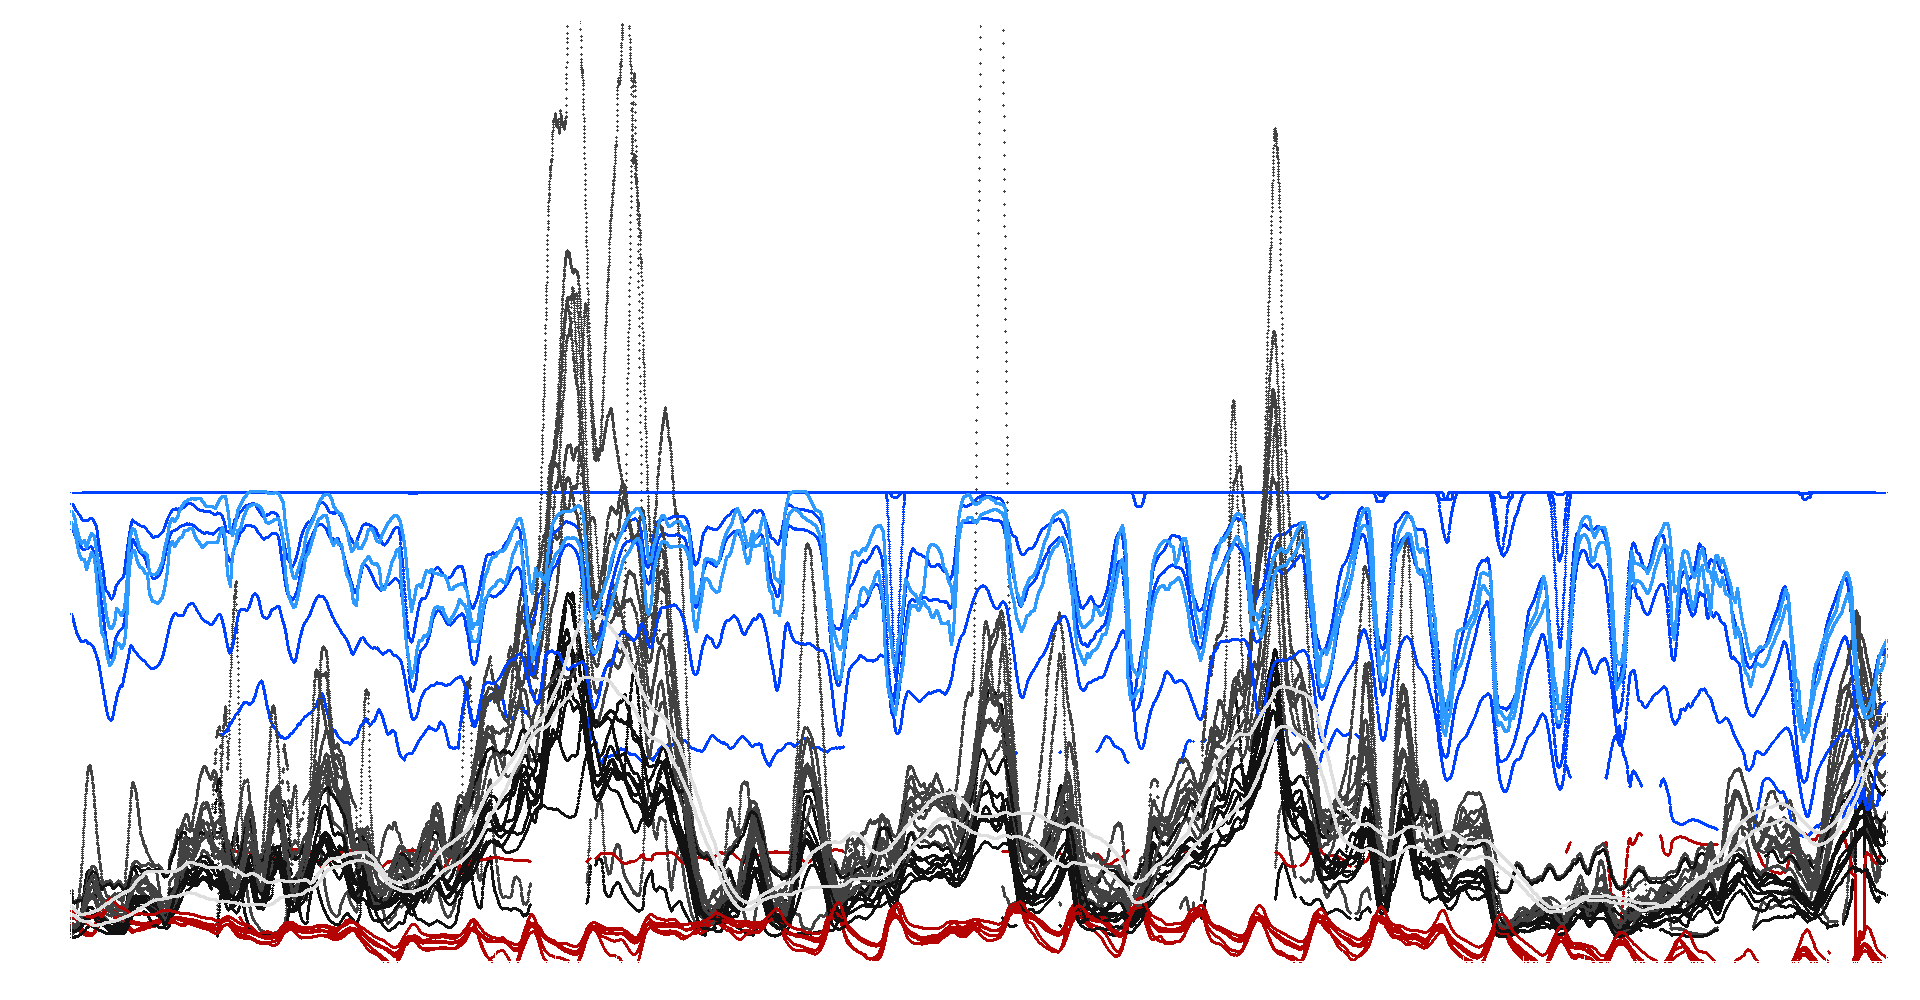
\includegraphics[width=\textwidth]{../png/2018-02-bs.png}
  \end{center}
\end{frame}
\begin{frame}{Hannover \hspace{4cm} Februar 2018}
  \begin{center}
    \includegraphics[width=\textwidth]{../png/2018-02-h.png}
  \end{center}
\end{frame}
\begin{frame}{Lehrte \hspace{2cm} Februar 2018}
  \begin{center}
    \includegraphics[width=\textwidth]{../png/2018-02-l.png}
  \end{center}
\end{frame}

\subsection{März}
\begin{frame}{Braunschweig März 2018}
  \begin{center}
    \includegraphics[width=\textwidth]{../png/2018-03-bs.png}
  \end{center}
\end{frame}
\begin{frame}{Hannover \hspace{4cm} März 2018}
  \begin{center}
    \includegraphics[width=\textwidth]{../png/2018-03-h.png}
  \end{center}
\end{frame}
\begin{frame}{Lehrte \hspace{2cm} März 2018}
  \begin{center}
    \includegraphics[width=\textwidth]{../png/2018-03-l.png}
  \end{center}
\end{frame}

\section*{Fazit}
\begin{frame}{Fazit?}
  \begin{itemize}
  \item offizielle Messtellen aussagekräfit genug?
  \item Lehrtes Feinstaub liegt \textbf{zwischen} Hannover und Braunschweig?
  \item offizielle Messpunkte reagieren langsam
  \item offizielle Messpunkte zeigen ``beruhigte'' Tagesschnitte
  \item offizielle Messpunkte an Silvester
  \end{itemize}
\end{frame}

\end{document}

